\todo[color=red]{move this to later, probably before depth interfacing}
Or more interestingly other sensors, such as depth or force sensors on robot hands or grippers (\todo{inspired by the MILES paper, talk about this}). This relates back to the idea of human perception. To learn new tasks, we use all kinds of feedback from the environment that is reactive on our actions. Therefore, it is important to study shortcomings of individual sensors with respect to others to understand how policies with limited access to sensors can be made to overcome such challenges without necessarily adding more `observability' to a workspace, which is the main problem we are trying to address with later active systems.\todo[color=blue]{reread and shorten if needed}


\section{Depth Interfacing}
Another area of important research, before relating all this back to active vision, is figuring out distance. Depth interfacing is an important part of perception. Continuing from the drawn parallels to humans, we place object in our fields of vision by our two eyes. Stereo-vision, allows us to process two slightly different poses of a target object to reinforce our understanding of where that object is in the environment around us. Other information such as lighting (shadows) may unconsciously help us as well. However, the main takeaway is that understanding distance to an object goes a long way in firstly understanding how to approach an object.

The few ways to achieve this in robotics and RLBench specifically is either to use two cameras (with a known distance between the two cameras to adjust poses with known intrinsics). However, RGB cameras are not the only things we have access to in this system. We also we have access to a depth sensor -and the point cloud information which is derived using this information.

This is because, as I hinted earlier in the background section, the main idea of active vision is to be able to use minimal amounts of viewpoints and make the most out of these. In this scenario, I want to see if it can be justified to use the wrist camera accompanied by the wrist depth sensor to replace any other cameras we might have around the workspace. Paving the way to the next section in proposing active vision policies that act solely on information from a repositionable sensor (be that rgb, depth or any other).

Therefore, I want to investigate whether depth data immediately adds meaningful information and if not; what is the best way to extract information from it so that it -combined with the normal rgb view- can be utilised to pave the way for active policies.

\subsection{Grasping with Varying Depths}
To start investigating, I devised the following test task to see how the agent reacts to differently sized targets that might be placed at varying distances from the gripper within the scene

\subsubsection{Task Design}
The experiment that makes sense in this case is a grasping task. Because unlike the reaching tasks from earlier, the robot will need slightly more precision in executing its grasp and actually grabbing the target. The task performer needs to figure out where an object is before attempting to grab it. So, I created a modified version of the simple grasping task where the target object's distance and scale can be externally varied to observe the behaviours of agents in a controlled manner.\todo[color=green]{talk about delegating the task creating and param passing as well as the tasks in appendix and link here}

\begin{figure}[htpb] % htpb allows all placement
  \centering
  \begin{subfigure}{0.4\linewidth}
    \centering
    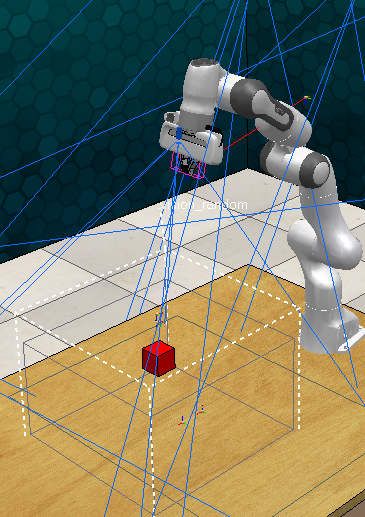
\includegraphics[width=0.7\linewidth]{assets/depth-interfacing/normal-size-grasp.png}
    \caption{Normal Target Size}\label{subfig:normal-grasp}
  \end{subfigure}
  \begin{subfigure}{0.4\linewidth}
    \centering
    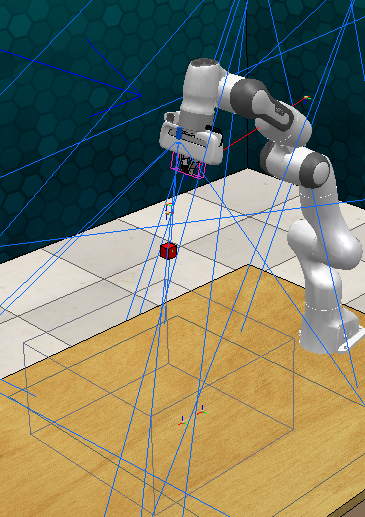
\includegraphics[width=0.7\linewidth]{assets/depth-interfacing/smaller-grasp.png}
    \caption{Smaller Target Size}\label{subfig:small-grasp}
  \end{subfigure}
  \caption{Visualisation of the Depth Interfacing experiment task}\label{fig:di-task}
\end{figure}

These, Figure \ref{fig:di-task}, is the general setup I am planning on using to evaluate the depth sensor versus a multi-view setup. 

\begin{figure}[htpb] % htpb allows all placement
  \centering
  \begin{subfigure}{0.4\linewidth}
    \centering
    
\includegraphics[width=0.7\linewidth]{assets/depth-interfacing/normal-size-wrist.png}
    \caption{Smaller - Wrist RGB}\label{subfig:normal-rgb}
  \end{subfigure}
  \begin{subfigure}{0.4\linewidth}
    \centering
    
\includegraphics[width=0.7\linewidth]{assets/depth-interfacing/smaller-wrist.png}
    \caption{Smaller - Wrist RGB}\label{subfig:small-rgb}
  \end{subfigure}
  \begin{subfigure}{0.40\linewidth}
    \centering
    
\includegraphics[width=0.7\linewidth]{assets/depth-interfacing/normal-depth.png}
    \caption{Wrist Depth Mask - Normal}\label{subfig:normal-depth}
  \end{subfigure}
  \begin{subfigure}{0.40\linewidth}
    \centering
    
\includegraphics[width=0.7\linewidth]{assets/depth-interfacing/smaller-depth.png}
    \caption{Wrist Depth Mask - Smaller}\label{subfig:small-depth}
  \end{subfigure}
  \caption{Wrist RGB and Depth Masks for the tasks}\label{fig:di-rgb-vs-depth}
\end{figure}

Initial observations from the side clearly indicate that these are two different targets and will require different reach lengths before the agent can attempt to grab them. However, as seen in the comparison in \ref{subfig:normal-rgb} and \ref{subfig:small-rgb}, the RGB outputs look practically the same, and will very likely produce extremely similar features after extraction. A way to differentiate them would be to utilise the wrist depth mask in this encoding. As shown in \ref{subfig:normal-depth} and \ref{subfig:small-depth}, they now carry different features in those areas. In the depth mask the darker colours indicate closer objects, and the information is encoded as floats. 

\begin{figure}[htpb] % htpb allows all placement
  \centering
  \begin{subfigure}{0.40\linewidth}
    \centering
    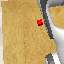
\includegraphics[width=0.7\linewidth]{assets/depth-interfacing/normal-l_rgb.png}
    \caption{Normal - Left Shoulder RGB}\label{subfig:normal-l-shoulder}
  \end{subfigure}
  \begin{subfigure}{0.40\linewidth}
    \centering
    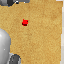
\includegraphics[width=0.7\linewidth]{assets/depth-interfacing/normal-r_rgb.png}
    \caption{Normal - Right Shoulder RGB}\label{subfig:normal-r-shoulder}
  \end{subfigure}
  \begin{subfigure}{0.40\linewidth}
    \centering
    
\includegraphics[width=0.7\linewidth]{assets/depth-interfacing/smaller-l_rgb.png}
    \caption{Smaller - Left Shoulder RGB}\label{subfig:smaller-l-shoulder}
  \end{subfigure}
  \begin{subfigure}{0.40\linewidth}
    \centering
    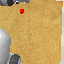
\includegraphics[width=0.7\linewidth]{assets/depth-interfacing/smaller-r_rgb.png}
    \caption{Smaller - Right Shoulder RGB}\label{subfig:smaller-r-shoulder}
  \end{subfigure}
  \caption{Left and Right Shoulder RGB Cameras}\label{fig:di-lr-shoulder}
\end{figure}


Another possible differentiating factor, and likely earlier tasks were performing well, is due to the shoulder cameras. These also provide extra information about the scene the agent can use to understand its 3D geometry, even if it isn't explicitly taught it. Although these are also not perfect, as seen in \ref{subfig:smaller-l-shoulder}, this camera is completely obstructed by the robot and is not seeing the target. This is not immediately problematic, because a smart enough system might be able to reason that the target is visible on the right and not on the left, leading to devising the correct depth for it. However, I have not intentionally encoded that information and doubt my network will be able to produce correct results with these observations.

\subsubsection{Adding Stereo Wrist Vision}\todo[color=red]{add wrist L and wrist R cameras, remove otherwise after a short mention}
A possibility to overcome this self-occlusion is to introduce stereo vision at the wrist level. Adding 2 off-centre cameras to the gripper, likely to the left and right of the existing wrist camera, will fix the self-occlusion, and possibly create a better comparison to the \emph{Wrist RGB} and \emph{Wrist Depth} combination. However, this comes with a lot of rewiring of RLBench and with its likely hidden issues that will pop up later. Will consider this further down the line, if there is evidence policies that will be proposed later can benefit form such a camera setup.



\subsubsection{Incorporating the Depth Camera to the previously introduced grasping}
probably cant just fuse with the rgb, might need a new conv for this then merger header

\todo{conclude depth here and move onto combination experiments}

